\subsection{Implementing Tests}
We have looked at how we built a repository of the adventure game in the section '\nameref{BuildRep}' and split it into pieces for the CLS. Here we will look at the same procedure of creating code, decomposing it and implementing it as combinators, just for the tests instead of the grains themselves. We want to be able to generate test cases that cover each of the game's variations, where only the needed tests are present in these, such that we can correctly test the variations, ensuring that they do indeed include the correct combinators and the game functions normally. \\
If we can synthesize testing with the CLS successfully, we should end up with the correct implementation of the grains and tests, such that all variations include thorough testing of their base implementation alongside tests specific to the current variation.  
\subsubsection{Player Unit Tests} \label{playerUnit}
The structure of units tests for the different grains are largely the same, except maybe for player. If we look at section '\nameref{BuildRep}' and subsection '\nameref{BuildPlayer}', we discussed the idea of dead code and modularization. In short, because of the high coupling between the grains, decomposition proved to be more difficult as we had not taken the high coupling into account earlier in the process. However, with tests it was both simpler per default and we had a focus on making it simple to decompose. \\
\begin{figure}[h]
    \centering
    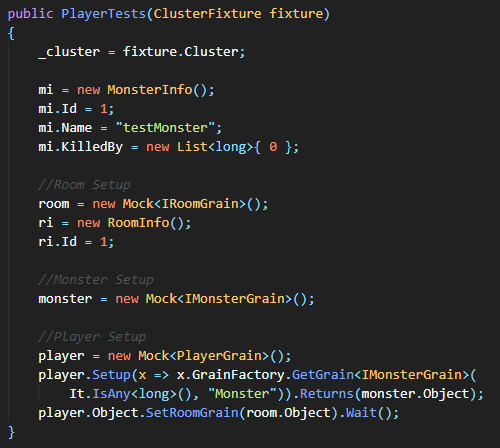
\includegraphics[width=0.7\linewidth]{Materials/TestingDiscussion/PlayerTestConstructor}
    \caption{The constructor for the player tests, showcasing how we chose to include the essentials for initialization.}
    \label{PlayerTestConstructor}
\end{figure}
If we look at \autoref{PlayerTestConstructor} we can see how we chose to setup the player tests. This setup is independent of the variation of the game we choose. Since we also have tests that are independent of variations, meaning they are included across all variations, the room mock and monster mock are initialized in the constructor. So, in tests that include the boss we chose to create the boss mock inside of those tests instead of in the setup alongside room and monster. There are two reasons for this. First off, as player does not include many boss tests we deemed it unnecessary to include in general setup. The second reason was to keep decomposition as simple as possible. If we keep the things affected by variations inside test cases we can decompose and combinate on a function level. This means, unlike in the grain decomposition, we do not have to insert lines of code here and there. This also means that the variations of abilities the player can take, fireball, roar and none, are not present in each others test. That is, for instance, fireball is not tested inside a damage test but these damage tests are kept separate. So, with this in mind, we can look at the CLS part of the tests and how we combinate those. \\
\\
Since tests of course are dependent on the grains, we can reuse some of the semantics from the grains. If we compare \autoref{semanticPlayerTest} to \autoref{SemanticTargetPlayer} from the subsection '\nameref{BuildPlayer}', we can see that they are similiar, however our semanticPlayerTestTargets differs in having another semantic type input in \textit{'playerTest}. 
\begin{figure}[h]
    \centering
    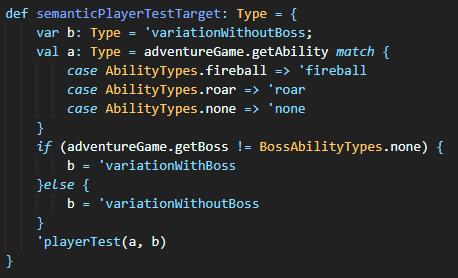
\includegraphics[width=0.7\linewidth]{Materials/TestingDiscussion/SemanticPlayerTestTarget}
    \caption{The function determining the semantic types for player tests.}
    \label{semanticPlayerTest}
\end{figure}
The reason we have the boss included in the semantic target is due to the fact that our player tests can be split in five parts. The first part of \autoref{semanticPlayerTest}, that is the pattern matching, would suffice for the first three parts of the player tests, which are the essential tests that will be included in all variations, the tests specific for roar and the tests specific for fireball. Then we have a test dealing damage to the boss. Most notably, one of our test cases include casting a fireball on the boss. That specific test is both dependent on a boss being present in the game variation and that the player ability is of type fireball. Only when those two criteria are fulfilled can we include that test. So with variations that vary both on the player's abilities and the presence of the boss, how did we combinate\todo{hedder det bare combine?} this? \\
\\
Before going into the semantics and structure of the player unit tests in our repository, we want to provide the reader with an overview of this structure, as it is somewhat complicated and a textual explanation may not suffice. We have provided a taxonomy of the player unit tests semantics, as can be seen in \autoref{taxonomyPlayerUnit}
\begin{figure}[H]
	\centering
	\begin{tikzpicture}[grow=down, -stealth]
	\node[bag]{Player Unit Test} 
	child[dashed]{;\node[bag]{testAbility}
		child[dashed]{; \node[bag]{bossPresent}
			child[dashdotted]{; \node[bag]{boss} % Dash eller solid?
				child[solid]{; \node[bag]{varWithBoss}}
			}
			child[solid]{; \node[bag]{varWithoutBoss}}	
		}
		child[solid]{; \node[bag]{fireball}}
		child[solid]{; \node[bag]{roar}}
		child[solid]{; \node[bag]{none}}
	};
	\end{tikzpicture}
	\caption{Taxonomy describing semantics of the player unit tests, showcasing the more complicated and nested structure.}
	\label{taxonomyPlayerUnit}
\end{figure}
It should be noted here that this is a simple representation of the structure and not a comprehensive one. For instance, both testAbility and bossPresent contain the two kindings, boss and ability. While this taxonomy looks similiar to \autoref{taxonomy}, with the same 'is a' and 'has a' connections, it differs slightly. Here we introduce a dash and dotted connection, which works as an optional 'has a'. This means that bossPresent either has a boss or is a varWithoutBoss, but not both at the same time. \\
\\ 
Semantically, we have split these combinators into three parts: \textit{'boss}, which contains the tests that are only dependent on the boss being a part of the game. That is, these tests do not use the player's abilities, but only the boss. The next semantic type is \textit{'bossPresent}. These combinators include tests that rely both on the player's ability and the boss. However, since we only have a single case where these overlap, it is only the \textit{'bossPresent('fireball, 'variationWithBoss)} that actually inserts a test, as there are no tests of roar and boss. The last semantic type is \textit{'testAbility} which contains the tests that are only specific for the player's ability. With these three parts, we can succesfully combinate all the possible variations of player tests that vary depending on ability and boss presence. Because of this, we can then describe player tests as: 
%\textit{string $\cap$ testAbility $\to$ MyResult $\cap$ playerTest}, where \textit{string $\cap$ boss $\to$ string $\cap$ bossPresent} and \textit{string $\cap$ bossPresent $\to$ string $\cap$ testAbility}
\begin{align*}
	&\textit{string $\cap$ testAbility} \to \textit{MyResult $\cap$ playerTest} \\
	\text{where\quad} &\textit{string $\cap$ bossPresent} \to \textit{string $\cap$ testAbility} \\
	\text{and\quad} &\textit{string $\cap$ boss} \to \textit{string $\cap$ bossPresent}
\end{align*}\todo{finno? ikke align?}
%\textit{string $\cap$ boss, string $\cap$ bossPresent, string $\cap$ testAbility $\to$ MyResult $\cap$ playerTest}\todo{forklar bedre? Er det korrekt? Nej, ikke helt så simpelt}. \\
This structure of the combinators is only due to the fireball boss test, which means that this intermediate step with the type of \textit{'bossPresent} is only truly meaningful when it comes to the fireball and boss variation. Because of this way we did the player tests, there are somewhat empty intermediate combinators for the abilities roar and none. That is, no tests are to be implemented that relies on the roar ability and the presence of the boss. We could argue that this opens up for the possibility of changing roar in a way that affects the boss, such that we needed tests that are dependent on these two. If this was the case, these new tests could easily be inserted into the intermediate combinator. However, we will not and do not expect roar to change in such a way to affect the boss directly, given the nature of the ability. This means that this structure of the player test combinators may seem somewhat redundant, due to the fact that the intermediate step, that is the intermediate combinators, is only needed for one specific case. So, if we were to look at the combinators of roar isolated, the intermediate step may seem irrelevant or puzzling.
\subsubsection{Room \& Boss Unit Tests}
Since neither room test nor boss tests have this overlap between multiple variables, it means that these tests are much simpler to implement. Let us start by looking at the boss tests. \\
\\
Boss tests are rather simple, as they only rely on the variation of the boss' abilities. Since boss does not take player or room into account, it makes for an easy synthesis. In essence, we only need one combinator for each of the boss' abilities for testing. Semantically, these combinators are of type \textit{'bossTest} that takes a kinding to specify which combinator to be chosen for synthesis. This means that boss tests can be described as: \textit{string $\cap$ bossTest $\to$ MyResult $\cap$ bossTestAbility}. However, this is not complete. \todo{Complete?} \\
The boss can have three different abilities: heal, DR (damage reduction) and none. The interesting ability here is none. None does not specify that the boss has no abilities, but instead it specifies that the boss is not present in this variation of the game. This means that the essential tests, that are independent of the boss' abilities, are no longer necessary and hence should not be included. This means in the case of no boss we do not need our \textit{'bossTest} to specify the tests that should be included based on abilities. This means we need a combinator that creates an empty file, such that no tests of the boss are present. This way, in the case where boss is nonexistent, boss tests can be described as: \textit{MyResult $\cap$ bossTestAbility}. \todo{Not sure how to show void $\to$ something. It would be intersected by 'none no?} \\
As the only factor of how the boss tests vary depends on the boss' abilities, tests of new abilities could easily be integrated as long as these tests are on a function level, such that this structure of \textit{'bossTest} can be kept. By doing this, scaling of the tests, based on new inclusion of abilities, seem feasible as the combinators do not intertwine and affect each other, a new combinator can simply be added for a given new ability. \todo{det er en kringle npnp. Lyder fint} %This also reinforces the idea that loose coupling makes for good combinators and thus this kind of unit testing is great in use of the CLS.
\\ \\
As the weather has been tested as its own class during unit testing, the room only need to take boss into account when being combinated. Other than the essential room tests, the only tests that vary from variation to variation is the boss part of room. This means that our semantic target for room only have two real cases, a \textit{'roomTestFile} with \textit{'boss} or with \textit{'noBoss}. Besides this, room is largely similiar to the boss tests in structure, where we have the semantic type \textit{'roomTest} that specifies a combinator with or without a boss. Therefore we can describe room tests as: \textit{string $\cap$ 'roomTest $\to$ MyResult $\cap$ 'roomTestFile}. 
\subsubsection{Integration Tests}
We have seen in \autoref{integrationDia} how we chose to implement integration testing with the bottom-up approach. The way we make integration tests is by testing one connection, for instance room and monster, then add player. This means that in PlayerIntegration tests we only test the remaining connections between the player, room and monster. This way, unlike unit tests, we no longer have to test the fireball / boss connection with player and boss in the PlayerIntegration, as this is now a connection to be tested when boss gets integrated, that is, during the BossIntegration. Because of this, player now only varies on the player abilities, as room and monster are default implementations that do not get altered \todo{hvad med weather tests? Godt spørgsmål :s}. So now PlayerIntegration is fairly simple to decompose and combinate, as we only have three non-overlapping cases to look at, that is the abilities: fireball, roar and none. The structure of PlayerIntegrationTests in our repository resembles the structure of the boss. Again, we have the semantic type \textit{'playerIntegrationAbility} of a given ability, that corresponds to the combinator that contains the tests specific for that ability. Since we kept the same structure as the unit tests, the essential tests that do not vary from variation to variation is already included in the file to be combinated, meaning that if we have \textit{'playerIntegrationAbility('none)} we get a combinator with an empty string, as no tests are to be added. We can describe PlayerIntegrationTests as: \textit{string $\cap$ 'playerIntegrationAbility $\to$ MyResult $\cap$ 'playerIntegration}. \\
%\\
%\begin{figure}[H]
%	\centering
%	\begin{tikzpicture}[grow=down, -stealth]
%	%\hspace{-2cm}
%	\node[bag]{Boss Integration Test} 
%	child[dashed]{;\node[bag]{bossIntegrationPlayerAbility}
%		child[solid]{; \node[bag]{None}}
%		child[solid]{; \node[bag]{Fireball}}
%	}
%	child[dashed]{;\node[bag]{bossIntegrationAbility}
%		child[solid]{; \node[bag]{DR}}
%		child[solid]{; \node[bag]{heal}}
%	};
%	\end{tikzpicture}
%	\caption{Taxonomy describing semantics of the boss integration tests, showcasing the simpler structure in comparison to the player unit tests.}
%	\label{taxonomyBossIntegration}
%\end{figure}
\begin{figure}[H]
	\centering
	\begin{tikzpicture}[grow=down, -stealth]
	\node[bag]{Boss Integration Test} 
	child[dashed]{;\node[bag]{bossIntAbility}
		child[dashed]{; \node[bag]{bossIntFireball}
			child[dashdotted]{; \node[bag]{ability} % Dash eller solid?
				child[solid]{; \node[bag]{fireball}}
			}
			child[solid]{; \node[bag]{none}}	
		}
		child[solid]{; \node[bag]{DR}}
		child[solid]{; \node[bag]{heal}}
		child[solid, thick]{; \node[bag]{none}}
	};
	\end{tikzpicture}
	\caption{Taxonomy describing semantics of the boss integration tests, showcasing how we have the same structure as our player unit tests.}
	\label{taxonomyBossIntegration}
\end{figure}
Now, since the connection of player and boss is tested during the BossIntegrationTests, this now resembles the same structure as the player unit tests. As with the playerTest, we have provided a diagram of bossIntegrationTests' taxonomy, which may help the reader more easily navigate the semantic structure as discussed. This can be seen in \autoref{taxonomyBossIntegration}. Here we have a new, thick line, which means that if bossIntAbility is a type none, we do not have a bossIntFireball connection. \\
In these boss integration tests, we need to take the player abilities into account, along with the boss abilities. Furthermore, because we may have a variation that does not contain the boss, we do not have boss unit tests and therefore we should neither have boss integration tests. This, just as in boss unit tests, also needs to be accounted for. 
As with the player unit tests, this structure requires the same intermediate step, because we have a test of the player fireball combined with the boss' damage reduction ability. If this was not the case, we would not require the intermediate step but rather have boss integration tests consisting of a player ability as well as a boss ability. In short, we have the same structure as player unit tests as we have the same overlap issue.
%However, we do not need the same intermediate step as in player unit tests, to account for the fireball boss test, as in this case, if we do not have a boss, we do not have boss integration tests at all and thus it is implied that if we do not combinate an empty boss integration file, we do indeed have a boss. 
%As such, tests that are dependent on specific player abilities can be combinated alongside the tests specific to boss abilities as these do not overlap as they did in player unit tests. 
\begin{figure}[]
    \centering
    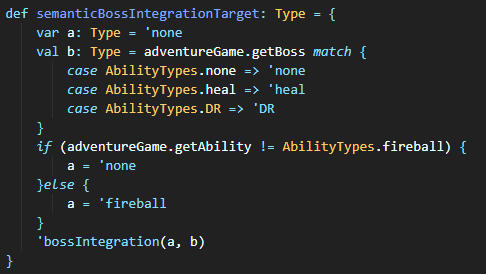
\includegraphics[width=0.6\linewidth]{Materials/TestingDiscussion/semanticBossIntegrationTarget}
    \caption{The function that specifies the boss' integration semantic targets, depending on boss abilities and player abilities.}
    \label{semanticBossIntegration}
\end{figure}
We can see in \autoref{semanticBossIntegration} the semantic target for boss integration tests. Here we can see, that like the player unit tests, we have an extra variable that depends on the player abilities. In this case, as we only have a connection between player and boss that depends on the player's fireball ability, we only have to check whether the variation includes this ability or not. However, it could easily be extended to a match case that includes the rest of the player abilities, if we made other abilities, or changed the current ones, such that other abilities than fireball had a connection with the boss and thus its integration tests. \\
Let us go over the semantics of boss integration tests. The tests specific to the player abilities, that is in our case either fireball or none, can be described as \textit{'bossIntegrationPlayerAbility}. The boss' abilities that include heal, DR and none are described as \textit{'bossIntegrationAbility}. The intermediate step, the tests depending on both player ability and boss ability are described as \textit{'bossIntegrationFireball}.
%With this in mind we can describe boss integration tests as: \textit{string $\cap$ 'bossIntegrationPlayerAbility, string $\cap$ 'bossIntegrationAbility $\to$ MyResult $\cap$ 'bossIntegration}. 
With this in mind, we can describe the boss integration tests the same way as player unit tests:
\begin{align*}
&\textit{string $\cap$ bossIntegrationAbility} \to \textit{MyResult $\cap$ bossIntegration} \\
\text{where\quad} &\textit{string $\cap$ bossIntegrationFireball} \to \textit{string $\cap$ bossIntegrationAbility} \\
\text{and\quad} &\textit{string $\cap$ bossIntegrationPlayerAbility} \to \textit{string $\cap$ bossIntegrationFireball}
\end{align*}
However, we also have the case with no boss integration tests at all, if we have any player ability, but the specific boss ability none. In this case, boss can simply be described as: \textit{MyResult $\cap$ 'bossIntegration}. \\
\\
In short, the way we chose to perform integration tests, the bottom-up approach, with the classes with least dependencies at the "bottom", proved to be the right choice as this made the integration tests easier for synthesis by implementing some connections later than others, that made for simpler combinators. However, we can see how the boss integration test has the same structure as the player unit tests, where both had to take each other into account due to the presence or abilities given, meaning that in this case, we only pushed this structure over to the boss integration tests instead of the player integration tests. \\
We can say that integration testing was a success synthesis-wise, atleast in our case with the adventure game, as all the integration tests made for fairly simple decomposing and combinators. This means that the tests are scalable, in the case of adding more variations to the game, atleast when it comes to the boss abilities and player abilities. However, just like with the unit tests, we still need to take care when it comes to overlaps, that is tests with multiple variation factors.
\subsubsection{Testing during Development}
So far, we have looked at how unit tests and integration testing has been implemented, decomposed and combinated with CLS, making tests that conform to specific variations of the adventure game. Let us take a step back and look at the tests more specifically for a moment. Now that we have made it clear how the tests have been incorporated into our repository, let us discuss more about the testing itself, what we have accomplished with it and how it has helped us doing development. \\
In \autoref{BuildRep} we discussed the implementation of grains in with CLS and how we came to the conclusion that accepting dead code would make it easier to decompose the grains. One may then ask, how do we ensure that this dead code is in fact unreachable or atleast how can we be sure that it does not create any obvious flaw in our variations where the dead code resides. More generally one could ask, how do our test overall ensure that our variations actually work as intended. \\ 
Let us examine the question, how can we somewhat reliably state that dead code does not crash our code? We can take the example of the dead code in \autoref{PlayerTakeDamage} that is, the if statement with roarActive inside player's TakeDamage function, in the variations where we do not have roar. We can see in \autoref{IntegrationTakeDamage} how we tested the player's takeDamage.
\begin{figure}[]
    \centering
    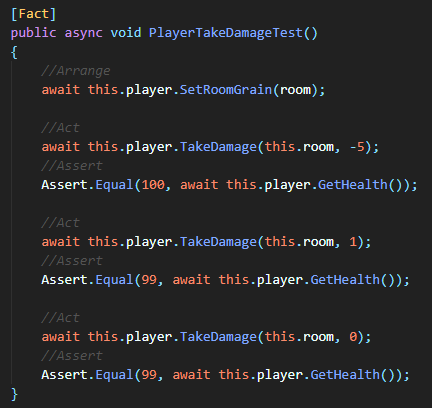
\includegraphics[width=0.6\linewidth]{Materials/TestingDiscussion/IntegrationTakeDamage}
    \caption{player's takeDamage in integration tests}
    \label{IntegrationTakeDamage}
\end{figure} 
As we only do black-box testing, we do not directly check the statements taken in TakeDamage while we test it. Instead, as we have mentioned in \autoref{TestTheory}, we use equivalence classes and boundary testing to examine how our TakeDamage reacts to different input. This way we cannot say that the dead code will never cause problems, but we have tested the function with input from our equivalence classes such that we can deem it unlikely that this code will affect the program with the input that we can expect the TakeDamage to receive doing runtime. \\ \\
Other than testing as an end product and as a result of synthesis, we can also look at how it helped us during development of our grains and their functionality. As we tested alongside development of our grains, the tests gave us valuable insight into problems or bugs that appeared as we implemented functionality, but also ways to simplify our code, which helped as a way to make grains simpler for decomposition \todo{hedder det decomposing?}. As a small example, originally the player was to implement a heal function, such that upon entering a sunny room, the player's heal function would be called. However, this was the only use for this function. As testing exposed the fact that we could take negative damage that would result in healing the player instead, we scrapped the heal function and used TakeDamage instead. \\
Even though we have used these black-box testing methods, our testing is not complete. As we will discuss in the next section, making tests with orleans and mockup did not go flawlessly and some of the functions proved difficult or downright impossible to test, atleast during unit testing. we will look at some of the obstacles that came during testing and what we did to work around or solve this in the next section. 
% Tests selv
%\subsubsection{Tests \& CLS}

